\documentclass[12pt]{article}
\usepackage[margin=1in]{geometry}
\usepackage{mathptmx}
\usepackage{parskip}
\usepackage{graphicx}
\usepackage{booktabs}
\usepackage{array}
\usepackage{hyperref}
\usepackage{setspace}
\usepackage{float}

\hypersetup{colorlinks=false, pdfborder={0 0 0}}
\onehalfspacing

\title{\textbf{NetStream}}
\author{Esko Qin, Awab}
\date{April 2025}

\begin{document}
\maketitle
\tableofcontents
\newpage

% ─────────────────────────────────────────────────────────────────────────────
\section{Introduction}

Modern streaming platforms adjust video quality automatically based on network speed. This is called Adaptive Bitrate Streaming (ABR). This project builds a working video streaming server from scratch and tests it under four simulated network conditions to find out which types of network problems actually cause quality drops, and which ones the system handles without the viewer noticing.

% ─────────────────────────────────────────────────────────────────────────────
\section{Background}

\subsection{How Streaming Works}

A video is split into short segments, each a few seconds long. The player downloads them one at a time while keeping a buffer of ready-to-play segments ahead of the current position. The buffer absorbs short slowdowns. If it empties, the video freezes.

\subsection{Bitrate and Quality Tiers}

Bitrate is how much data per second a video needs to play at a given resolution. This project uses two tiers:

\begin{center}
\begin{tabular}{lll}
\toprule
Quality & Resolution & Required Bitrate \\
\midrule
Low  & 360p & 500 kbps   \\
High & 720p & 2,500 kbps \\
\bottomrule
\end{tabular}
\end{center}

If bandwidth falls below 2,500 kbps, the player must switch to 360p or risk buffering.

\subsection{Adaptive Bitrate Streaming and HLS}

HLS (HTTP Live Streaming) encodes a video into multiple quality versions, each split into segment files. A master playlist lists all versions and their bandwidth requirements. The player, hls.js, reads this playlist, measures download speed after each segment, and switches quality tiers automatically to match the available bandwidth.

\subsection{Types of Network Problems}

\textbf{Latency} adds delay to every packet. Segments start arriving later but data flows at full speed once transmission begins. Total throughput is not reduced.

\textbf{Packet loss} drops some packets. TCP detects this and retransmits them automatically. The data eventually arrives, but retransmissions add extra time.

\textbf{Bandwidth cap} sets a hard limit on data per second. Unlike delay or loss, it cannot be compensated for. If the cap is below what a quality tier needs, that tier cannot be sustained.

\subsection{tc netem}

tc netem is a Linux kernel tool that injects delay, packet loss, or bandwidth caps into a network interface at the OS level. TCP sees these as real conditions, so the streaming system responds exactly as it would on a degraded connection.

% ─────────────────────────────────────────────────────────────────────────────
\section{Project Goal}

Build a complete HLS streaming system, apply four network conditions using tc netem, and measure which conditions cause the player to drop video quality.

% ─────────────────────────────────────────────────────────────────────────────
\section{System Implementation}

\subsection{Architecture}

The server runs inside Ubuntu WSL2 on Windows 11. The browser is Windows Chrome, connecting to the server at localhost:3000. tc netem rules are applied to the WSL2 loopback interface, which carries all Chrome-to-server traffic in this environment.

\subsection{Server}

Built with Node.js and Express. Uploaded videos are passed to FFmpeg, which encodes two HLS renditions simultaneously: 360p at 500 kbps and 720p at 2,500 kbps, each split into 4-second segments. After encoding, a master playlist is written listing both renditions.

FFmpeg is launched using Node.js \texttt{spawn()} rather than \texttt{exec()}. \texttt{exec()} buffers all FFmpeg output in memory and crashes on long videos. \texttt{spawn()} streams it without storing it.

\subsection{Browser Frontend}

The upload page sends files to the server and polls the status endpoint until processing is complete. The player page loads hls.js from a CDN and plays the video using the master playlist. A stats panel updates every second showing quality level, bandwidth estimate, buffer length, and switch count. An auto-recorder captures a snapshot every 30 seconds for three minutes and exports a CSV.

\subsection{Network Simulation}

netem.sh applies tc netem rules to the loopback interface. It clears any existing rules before each profile.

\begin{center}
\begin{tabular}{>{\raggedright}p{2.6cm} >{\raggedright}p{3.8cm} l l}
\toprule
Profile & Delay & Packet Loss & Bandwidth Cap \\
\midrule
Baseline     & 0 ms                     & 0\% & None      \\
High Latency & 150 ms                   & 0\% & None      \\
Packet Loss  & 0 ms                     & 3\% & None      \\
Congested    & 200 ms $\pm$30 ms jitter & 2\% & 1.5 Mbps  \\
\bottomrule
\end{tabular}
\end{center}

The congested profile uses 200 ms delay with $\pm$30 ms jitter rather than a small fixed value. Normal internet latency across a continent is 60--80 ms, so a low fixed delay would resemble an ordinary connection. Jitter reflects real congestion, where router queue occupancy fluctuates and packet arrival times vary.

% ─────────────────────────────────────────────────────────────────────────────
\section{Experiment Design}

The same gameplay video clip was used for all four runs. It loops automatically since it is shorter than three minutes. For each run: the server was restarted, the player page opened with cache disabled, the profile applied, and the auto-recorder started immediately on playback. The browser tab was kept visible throughout — background tabs throttle JavaScript timers and would corrupt the data.

\subsection{Collected Data}

Six samples were taken per profile at 30-second intervals. Quality and bandwidth were stable within each profile, so the table shows a single representative value. Total switches are the final cumulative count at t=180s.

\begin{center}
\begin{tabular}{lrrl}
\toprule
Profile & Bandwidth (kbps) & Total Switches & Quality \\
\midrule
Baseline     & 369,257 & 7 & 720p \\
High Latency &  69,755 & 7 & 720p \\
Packet Loss  & 207,238 & 7 & 720p \\
Congested    &   1,457 & 0 & 360p \\
\bottomrule
\end{tabular}
\end{center}

% ─────────────────────────────────────────────────────────────────────────────
\section{Results}

\begin{figure}[H]
\centering
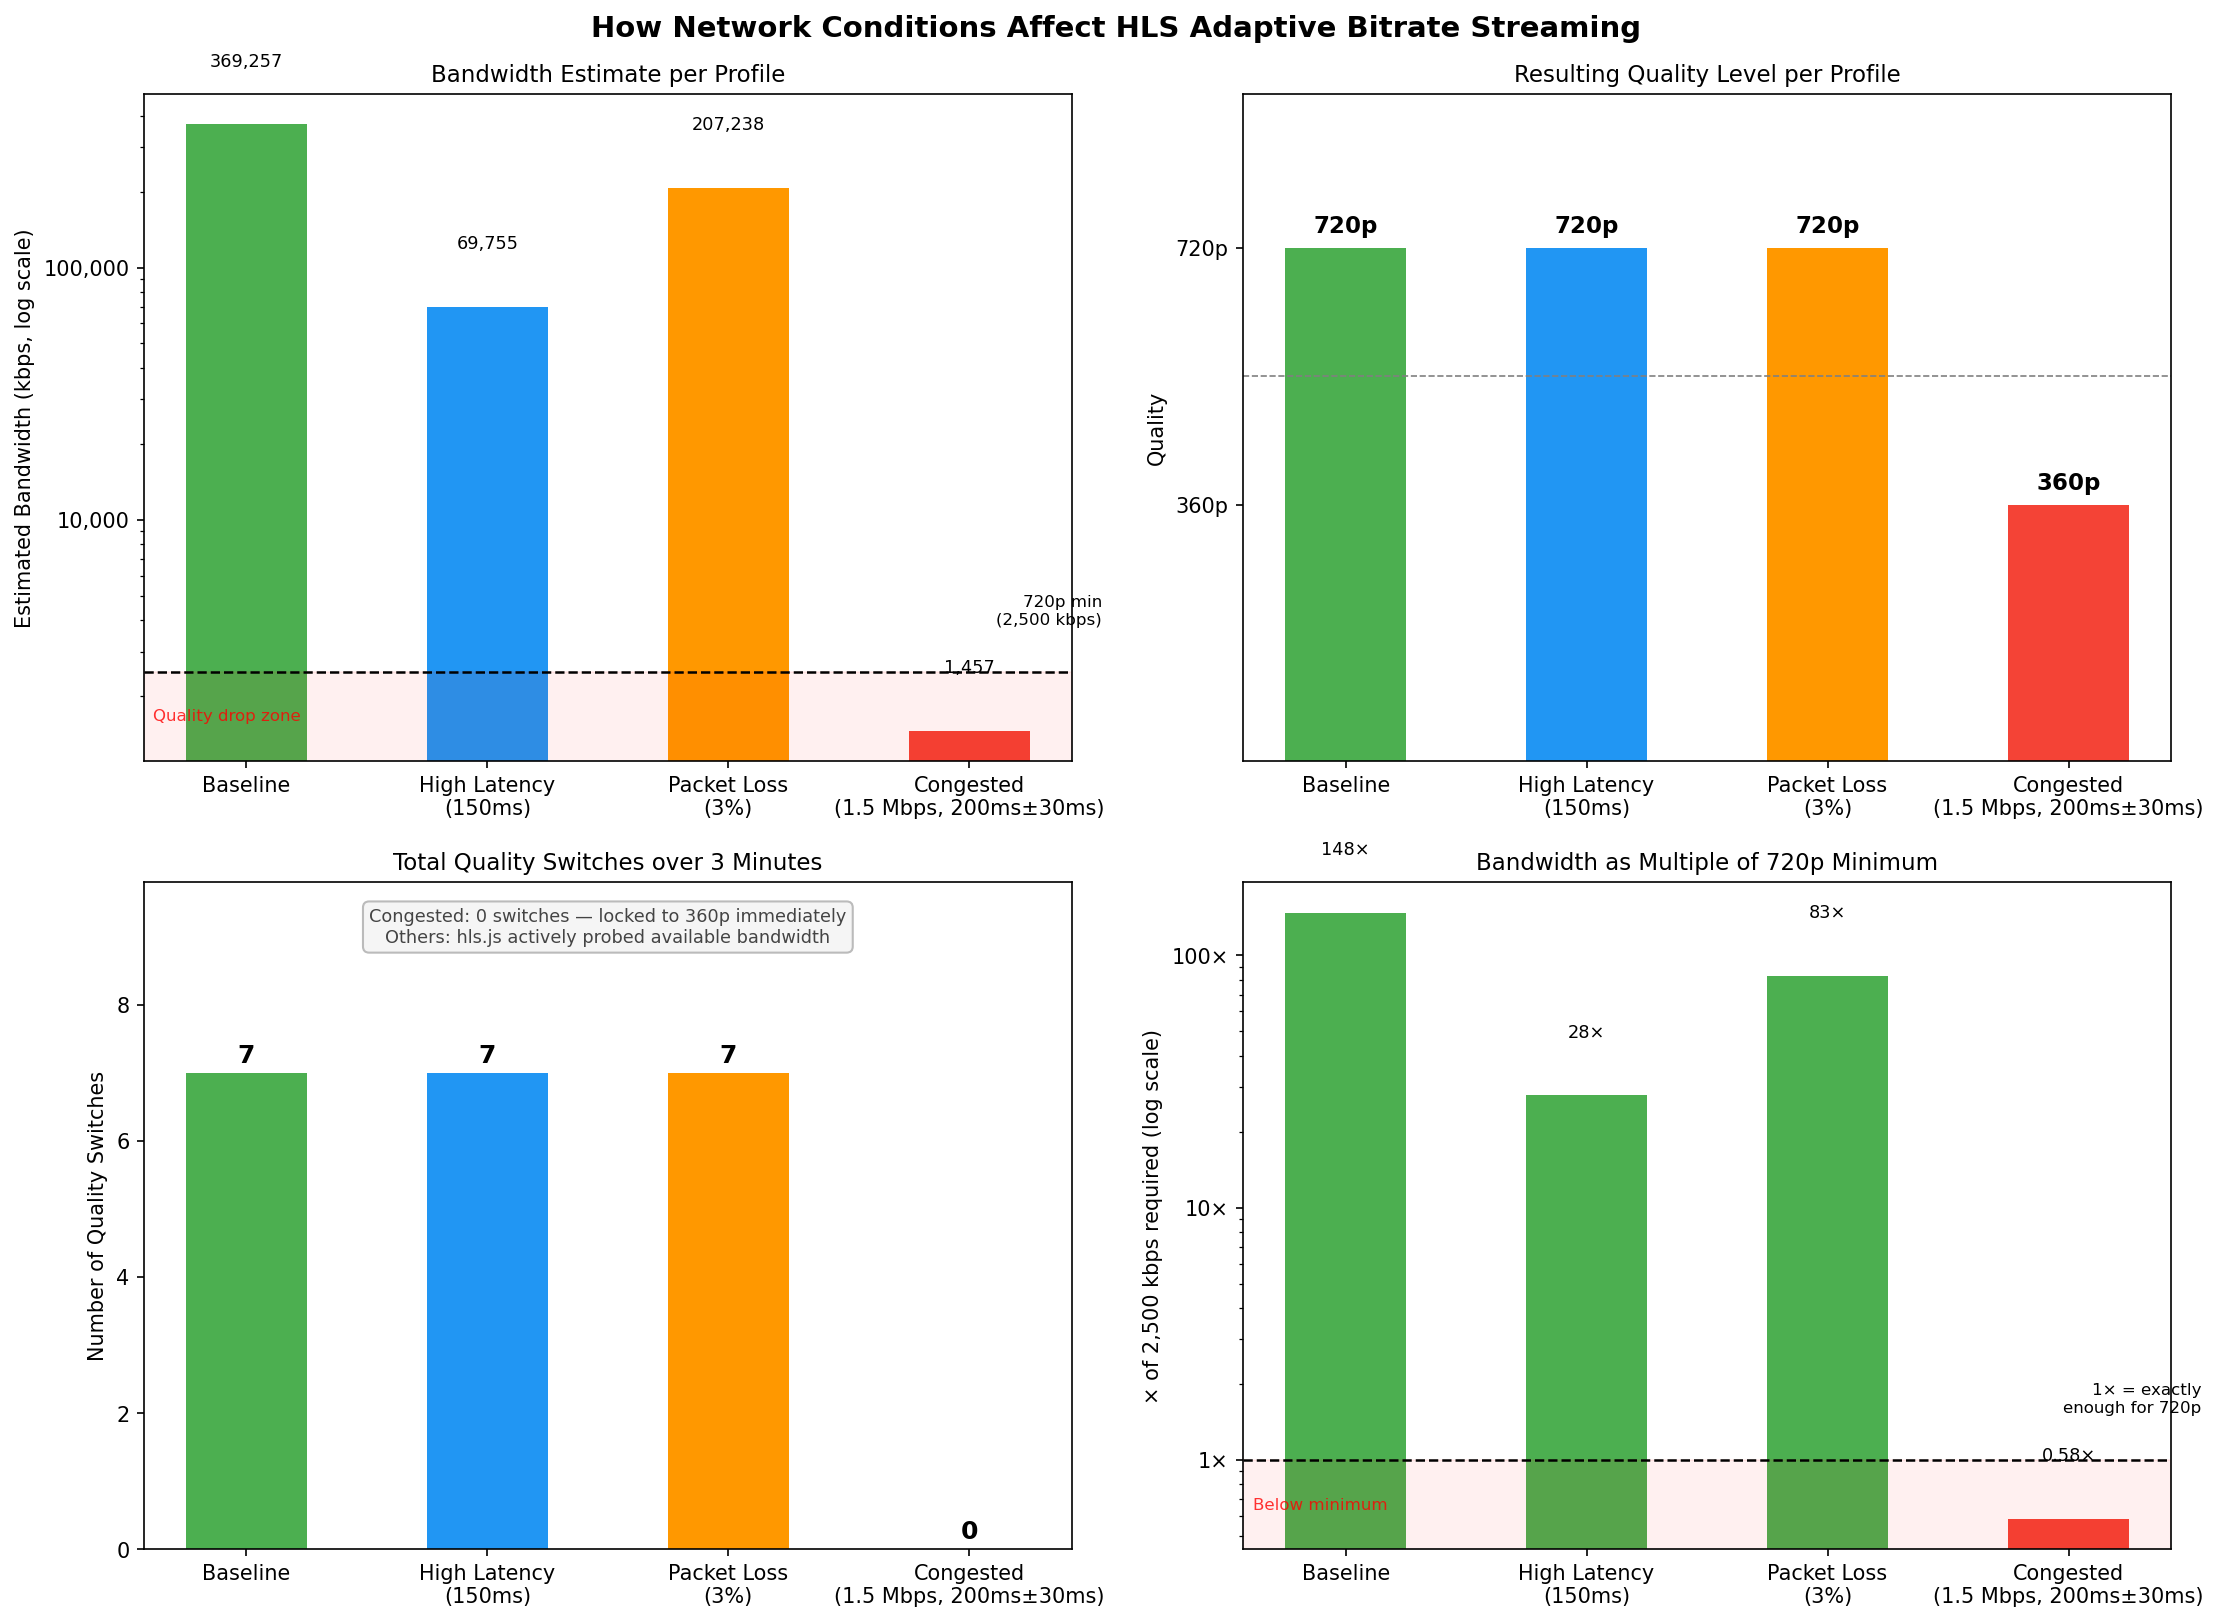
\includegraphics[width=\textwidth]{../data/charts.png}
\caption{Top left: bandwidth estimate per profile (log scale), dashed line at the 2,500 kbps minimum for 720p. Top right: quality level per profile. Bottom left: total quality switches over three minutes. Bottom right: bandwidth as a multiple of the 720p minimum, dashed line at 1$\times$.}
\end{figure}

The top-left chart shows the bandwidth hls.js measured under each profile. The log scale is needed because the range spans 250 to 1 --- from 369,257 kbps at baseline to 1,457 kbps under congestion. Three profiles sit above the 2,500 kbps threshold. Only congested falls below.

The top-right chart shows the resulting quality. Baseline, latency, and loss stayed at 720p for all six samples. Congested locked to 360p from the first sample.

The bottom-left chart shows quality switches. The three non-congested profiles each ended at 7 switches as hls.js adjusted over time. Congested produced 0 --- the player made one decision and never reconsidered.

The bottom-right chart shows bandwidth as a multiple of the 720p minimum. Baseline, latency, and loss sit at 148$\times$, 28$\times$, and 83$\times$. Congested sits at 0.58$\times$ --- the only profile below 1$\times$.

% ─────────────────────────────────────────────────────────────────────────────
\section{Analysis}

\subsection{Latency}

Adding 150 ms of delay reduced the measured bandwidth from 369,257 to 69,755 kbps, an 80\% drop. But 69,755 kbps is still 28 times the 720p threshold. hls.js had no reason to switch. Delay slows when each segment starts arriving, not the speed at which data flows once transmission begins.

\subsection{Packet Loss}

Dropping 3\% of packets reduced bandwidth from 369,257 to 207,238 kbps. TCP retransmitted every lost packet, so all data arrived. The retransmissions added variable delay, which lowered the bandwidth estimate, but 207,238 kbps is 83 times the threshold. No switches, no stalls. The loss was invisible to the player.

\subsection{Congestion}

The 1.5 Mbps cap placed a hard ceiling of 1,500 kbps on throughput. The 720p tier needs 2,500 kbps. That gap cannot be closed by retransmissions or buffering. hls.js measured 1,457 kbps, saw it was below the threshold, and selected 360p before the first sample. Quality stayed at 360p for the full three minutes with zero switches. The 0 switch count is also notable: with 360p fitting comfortably inside the cap, the player had no reason to probe a higher tier.

\subsection{Core Finding}

Network degradation alone does not cause a quality drop. What matters is whether throughput falls below the minimum required for the current tier. Latency and loss are forms of degradation TCP can absorb. A bandwidth cap is not --- and the ABR system responds to it exactly as designed.

% ─────────────────────────────────────────────────────────────────────────────
\section{Limitations}

All traffic ran over the loopback interface within a single machine. Real-world factors --- routing hops, physical link noise, shared congestion --- are absent. Results are reproducible but describe idealized conditions, not live internet behavior. Only one video clip and two quality tiers were tested.

% ─────────────────────────────────────────────────────────────────────────────
\section{Conclusion}

This project built a working HLS streaming server, applied four network conditions with tc netem, and measured how hls.js responded to each one. The finding is clear: ABR is sensitive to bandwidth constraints, not network degradation in general. Latency and packet loss were absorbed by TCP and the player buffer with no quality change. Only a bandwidth cap below the minimum threshold forced a quality drop --- exactly the behavior ABR is designed to produce.

\end{document}
